\documentclass{article}

\usepackage{graphicx}
\usepackage{amsfonts,amsmath,amssymb,amsthm}
\usepackage{url}
\usepackage[usenames]{color}

\newcommand{\figref}[1]{Figure~\ref{#1}}

\pagestyle{empty} \addtolength{\textwidth}{1.0in}
\addtolength{\textheight}{0.5in} \addtolength{\oddsidemargin}{-0.5in}
\addtolength{\evensidemargin}{-0.5in}
\newcommand{\ruleskip}{\bigskip\hrule\bigskip}
\newcommand{\nodify}[1]{{\sc #1}} \newcommand{\points}[1]{{\textbf{[#1
points]}}}

\newcommand{\bitem}{\begin{list}{$\bullet$}%
{\setlength{\itemsep}{0pt}\setlength{\topsep}{0pt}%
\setlength{\rightmargin}{0pt}}} \newcommand{\eitem}{\end{list}}

\input{../../defs}

\newcommand{\G}{\mathcal{G}}

%\newcommand{\bE}{\mbox{\boldmath $E$}}
%\newcommand{\be}{\mbox{\boldmath $e$}}
%\newcommand{\bU}{\mbox{\boldmath $U$}}
%\newcommand{\bu}{\mbox{\boldmath $u$}}
%\newcommand{\bQ}{\mbox{\boldmath $Q$}}
%\newcommand{\bq}{\mbox{\boldmath $q$}}
%\newcommand{\bX}{\mbox{\boldmath $X$}}
%\newcommand{\bY}{\mbox{\boldmath $Y$}}
%\newcommand{\bZ}{\mbox{\boldmath $Z$}}
%\newcommand{\bx}{\mbox{\boldmath $x$}}
%\newcommand{\by}{\mbox{\boldmath $y$}}
%\newcommand{\bz}{\mbox{\boldmath $z$}}

\newcommand{\true}{\mbox{true}}
\newcommand{\Parents}{\mbox{Parents}}

\newcommand{\ww}{{\bf w}}
\newcommand{\xx}{{\bf x}}
\newcommand{\yy}{{\bf y}}
\newcommand{\real}{\ensuremath{\mathbb{R}}}


\newcommand{\eat}[1]{}

\newcommand{\CInd}[3]{({#1} \perp {#2} \mid {#3})}
\newcommand{\Ind}[2]{({#1} \perp {#2})}

\setlength{\parindent}{0pt} \setlength{\parskip}{0.5ex}

\begin{document}

\pagestyle{myheadings} \markboth{}{DS-GA-1005/CSCI-GA.2569 Problem Set
  3 -- Due Tuesday, Oct 10 }

{\LARGE
\begin{center}Inference and Representation, Fall 2017\end{center}
}

{\Large
Problem Set 3: Gibbs Sampling,  Belief Propagation, Tree Structure Learning
}


%{\bf Selected solutions}\\
\ruleskip 
{\em You are allowed to use basic graph packages (e.g., for representing
and working with undirected graphs, or for finding the maximum
spanning tree), but are {\bf not} permitted to use any machine learning, graphical models, or probabilistic inference packages. }

%\vspace{0.2in}

\begin{enumerate}

\item {\bf Ising Model - Gibbs sampling (\cite{blitzstein2014introduction} Ex. 12.5.3(a)).}

This problem considers an application of MCMC techniques to image analysis. Imagine a 2D image consisting of an $L\times L$ grid of black-or-white pixels. Let $Y_j$ be the indicator of the $j$th pixel being white, for $j = 1,..., L^2$. Viewing the pixels as nodes in a network, the neighbors of a pixel are the pixels immediately above, below, to the left, and to the right (except for boundary cases).

Let $i \sim j$ stand for "$i$ and $j$ are neighbors". A commonly used model for the joint PMF
of $Y = (Y_1,... , Y_{L^2})$ is
$$P(Y = y) \propto \exp (\beta \sum_{(i,j): i \sim j} I(y_i = y_j))$$
If $\beta$ is positive, this says that neighboring pixels prefer to have the same color. The normalizing constant of this joint PMF is a sum over all $2^{L^2}$
possible configurations, so it may be very computationally difficult to obtain. This motivates the use of MCMC to
simulate from the model.

Suppose that we wish to simulate random draws from the joint PMF of $Y$ for a particular known value of $\beta$. Explain how we can do this using Gibbs sampling, cycling
through the pixels one by one in a fixed order.

\item {\bf Sum-product algorithm, Homework 1 in \cite{Brown} adapted to Python.} We implement the sum-product variant of the belief propagation algorithm to compute marginals. To understand the details of the sum-product algorithm, we recommend Chapter 5 of Barber's "Bayesian Reasoning and Machine Learning", as well as "Factor Graphs and the Sum-Product Algorithm" by Kschischang, Frey, \& Loeliger, IEEE Trans. Information Theory 47, pp. 498-519, 2001.

You must write your own novel implementation of the sum-product algorithm in Python, not copy code from other students or existing software packages.

We  provided code implementing a data structure to store the graph adjacency structure, and numeric potential tables, defining any discrete factor graph. We also provided code that explicitly builds a table containing the probabilities of all joint configurations of the variables in a factor graph, and sums these probabilities to compute the marginal
distribution of each variable. Such "brute force" inference code is of course inefficient, and will only be computationally tractable for small models.

We recommend (but do not require) that you use these same data structures for your own implementation of the sum-product algorithm, by implementing \path{run_loopy_bp_parallel}
and \path{get_beliefs}. To gain intuition for the graph structure, examine the output of \path{make_debug_graph.ipynb}. Think of the code we provide as a starting point: you are welcome to create additional functions or data structures as needed. 

\begin{enumerate}
\item Implement the sum-product algorithm. Your code should support an arbitrary factor graph linking a collection of discrete random variables. Use a parallel message update schedule,
in which all factor-to-variable messages are updated given the current variable-to-factor messages, and then all variable-to-factor messages given the current factor-to-variable
messages. Initialize by setting the variable-to-factor messages to equal 1 for all states.
Be careful to normalize messages to avoid numerical underflow.


\item Consider the four-node, tree-structured factor graph illustrated in Figure \ref{fig:tree} with binary variables. Numeric values for the potential functions are defined in \path{make_debug_graph.ipynb}. Run your implementation of the sum-product algorithm on this graph, and report the marginal distributions it computes. Verify that these are consistent with the results of \path {marg_brute_force.ipynb}.
\begin{figure}[t]
\centering
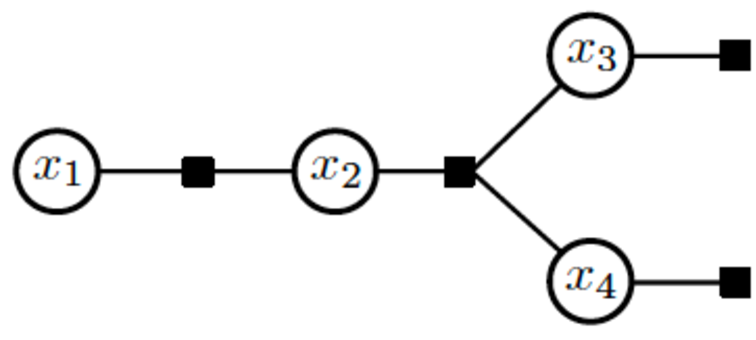
\includegraphics[width=2in]{brown_hw1}
\caption{A tree-structured factor graph in which four factors link four random variables. Variable
$x_2$ takes one of three discrete states, and the other three variables are binary. \cite{Brown}}
\label{fig:tree}
\end{figure}
\end {enumerate}

\item  {\bf LDPC, Homework 2 in \cite{Brown} adapted to Python.} We begin by designing algorithms for reliable communication in the presence of noise. We
focus on error correcting codes based on highly sparse, low density parity check (LDPC) matrices, and use the sum-product variant of the loopy belief propagation (BP) algorithm
to estimate partially corrupted message bits. For background information on LDPC codes, see Chap. 47 of MacKay's Information Theory, Inference, and Learning Algorithms, which
is freely available online: \url{http://www.inference.phy.cam.ac.uk/mackay/itila/}.

We consider rate 1/2 error correcting codes, which encode N message bits using a 2N-bit codeword. LDPC codes are specified by a $N \times 2N$ binary parity check matrix H,
whose columns correspond to codeword bits, and rows to parity check constraints. We define $H_{ij} = 1$ if parity check $i$ depends on codeword bit $j$, and $H_{ij} = 0$ otherwise. Valid codewords are those for which the sum of the bits connected to each parity check, as indicated by H, equals zero in modulo-2 addition (i.e., the number of "active" bits must be even). Equivalently, the modulo-2 product of the parity check matrix with the 2N-bit codeword vector must equal a N-bit vector of zeros. As illustrated in Figure \ref{fig:factor}, we can visualize these
parity check constraints via a corresponding factor graph. The parity check matrix H can then be thought of as an adjacency matrix, where rows correspond to factor (parity) nodes,
columns to variable (codeword bit) nodes, and ones to edges linking actors to variables.

\begin{figure}[t]
\centering
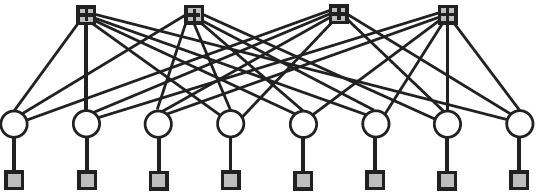
\includegraphics[width=2in]{brown_hw2}
\caption{A factor graph representation of a LDPC code linking four factor (parity constraint)
nodes to eight variable (message bit) nodes. The unary factors encode noisy observations of the
message bits from the output of some communications channel. \cite{Brown}}
\label{fig:factor}
\end{figure}

\begin{enumerate}
\item Implement code that, given an arbitrary parity check matrix H, constructs a corresponding factor graph. The parity check factors should evaluate to 1 if an even number of adjacent bits are active (equal 1), and 0 otherwise. Your factor graph representation should interface with your implementation of the sum-product algorithm from the previous problem. Define a small test case, and verify that your graphical model assigns zero probability to invalid codewords.
\item Load the $N = 128$-bit LDPC code using the Python library \path{pyldpc} (for a tutorial see \url {github.com/hichamjanati/pyldpc-tutos}).  To evaluate decoding
performance, we assume that the all-zeros codeword is sent, which always satisfies any set of parity checks. Using the random module, simulate the output of a binary symmetric
channel: each transmitted bit is flipped to its complement with error probability $\epsilon =0.05$, and equal to the transmitted bit otherwise. Define unary factors for each variable node
which equal $1-\epsilon$ if that bit equals the "received" bit at the channel output, and $\epsilon$ otherwise. Run the sum-product algorithm for 50 iterations of a parallel message update schedule, initializing by setting all variable-to-factor messages to be constant. After the final iteration, plot the estimated posterior probability that each codeword bit equals one.
If we decode by setting each bit to the maximum of its corresponding marginal, would we find the right codeword?
\item Repeat the experiment from part (b) for 10 random channel noise realizations with error probability $\epsilon= 0.06$. For each trial, run sum-product for 50 iterations. After each iteration, estimate the codeword by taking the maximum of each bit's marginal distribution, and evaluate the Hamming distance (number of differing bits) between the estimated and true (all-zeros) codeword. On a single plot, display 10 curves showing Hamming distance versus iteration for each Monte Carlo trial. Is BP a reliable decoding algorithm?
\item Repeat part (c) with two higher error probabilities, $\epsilon = 0.08$ and $\epsilon = 0.10$. Discuss any qualitative differences in the behavior of the loopy BP decoder.
\item For the LDPC codes we consider, we also define a corresponding $2N\times N$ generator matrix G. To encode an N-bit message vector we would like to transmit, we take the modulo-2 matrix product of the generator matrix with the message. The generator matrix has been constructed (via linear algebra over the  finite field GF(2)) such that this product always produces a valid 2N-bit codeword. Geometrically, its columns are chosen to span the null space of H. We use a systematic encoding, in which the first N codeword bits are simply copies of the message bits. The problems below use precomputed (G;H) pairs using the relevant functions in  \path{pyldpc}. Generate the $N = 1600$-bit LDPC code. Using this, we will replicate the visual decoding demonstration from MacKay's Fig. 47.5. Start by converting a $40\times 40$ binary image to a 1600-bit message vector; you may use the \path{logo} image we provide, or create your own. Encode the message using the  generator matrix $G$,
and add noise with error probability $\epsilon = 0.06$. For this input, plot images showing the output of the sum-product decoder after 0, 1, 2, 3, 5, 10, 20, and 30 iterations. The \%
operator may be useful for computing modulo-2 sums. You can use the numpy reshape function to easily convert between images and rasterized message vectors.
\item Repeat the previous part with a higher error probability of $\epsilon =0.10$, and discuss differences.
\end{enumerate}


\item {\bf Chow-Liu algorithm.} When trying to do object detection from computer images, {\em context} can be very helpful. For example, if "car" and "road" are present in an image, then it is likely that "building" and "sky'" are present as well (see Figure~\ref{fig:object_rec}). In recent work, a tree-structured Markov random field (see Figure~\ref{fig:object_rec2}) was shown to be particularly useful for modeling the prior distribution of what objects are present in images and using this to improve object detection \cite{choi_cvpr10}.
\begin{figure}[t]
\centering
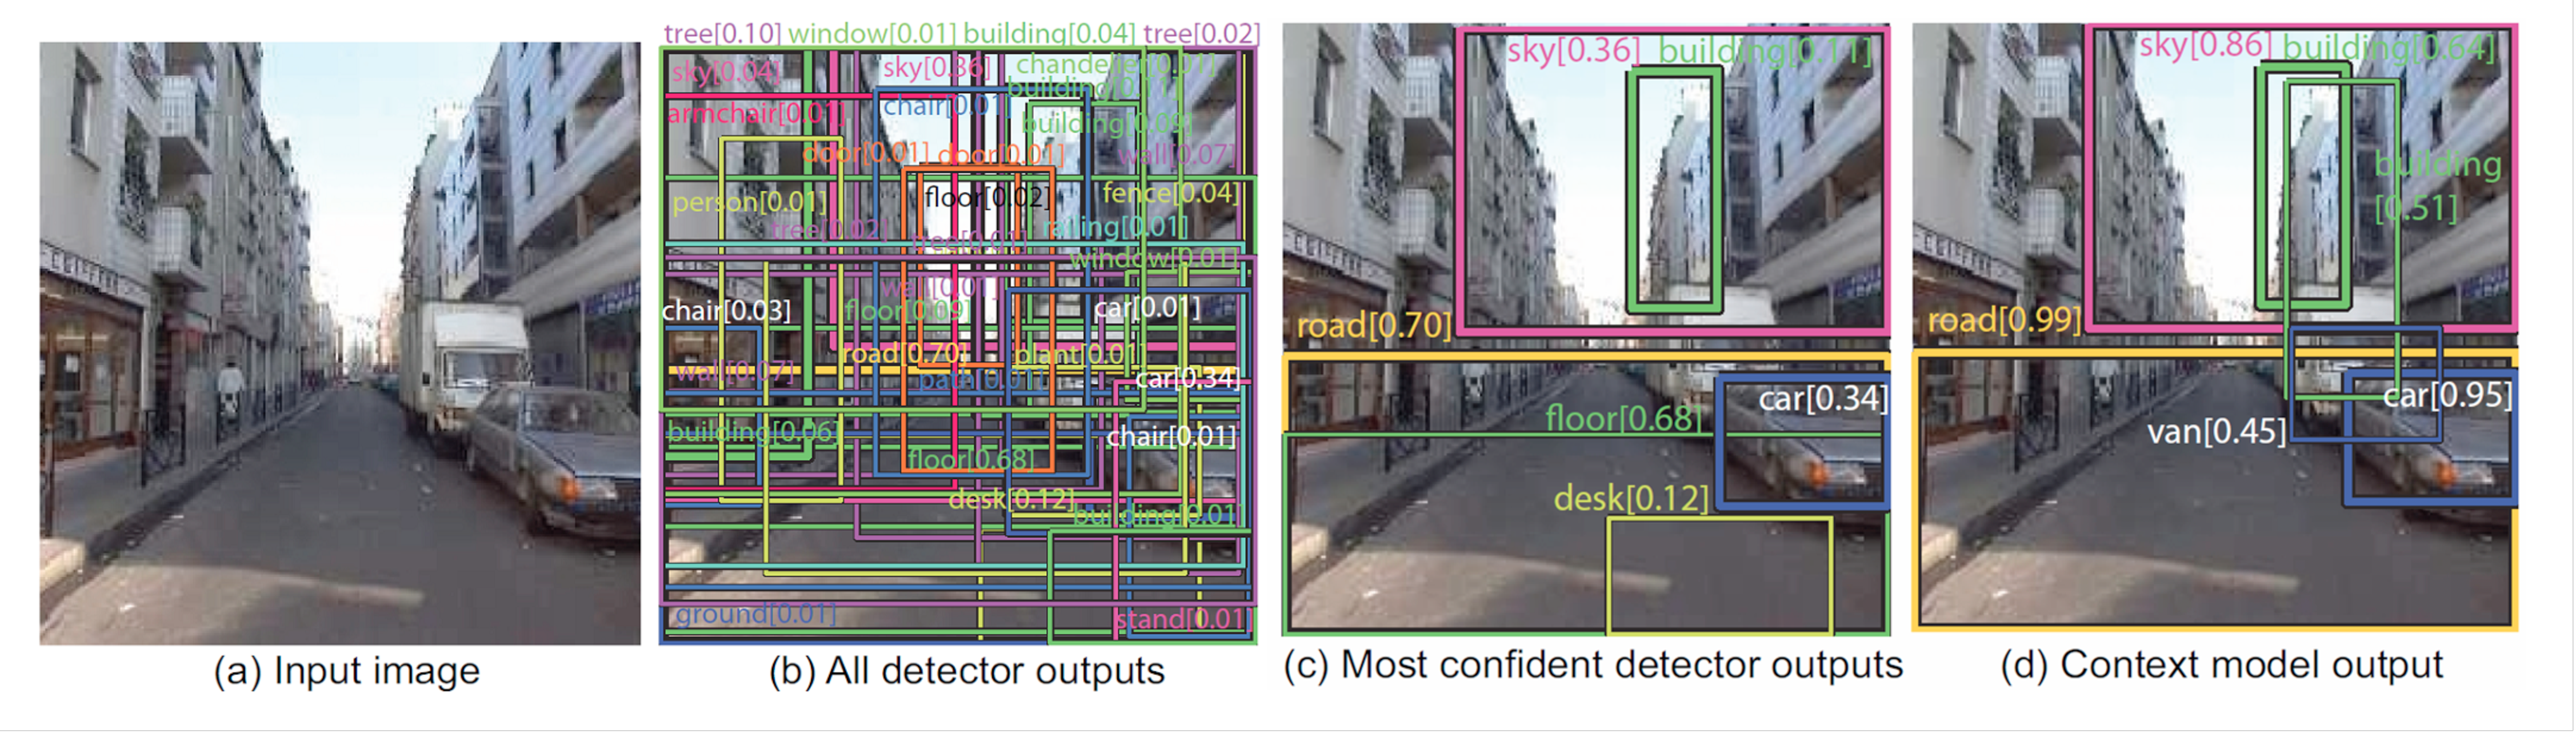
\includegraphics[width=5.8in]{object_recognition_in_context}
\vspace{-8mm}
\caption{Using context within object detection for computer vision. \cite{choi_cvpr10}
\label{fig:object_rec}}
\end{figure}

You will replicate some of the results from
\cite{choi_cvpr10} (it is not necessary to read this paper to complete
this assignment).
%\footnote{That said, please see \url{http://people.csail.mit.edu/myungjin/HContext.html} if you are curious for more details. We omit the spatial prior and the global image features, and use only the co-occurences prior and the local detector outputs ($b_i, c_{ik}, \textrm{and } s_{ik}$ from \cite{choi_cvpr10}'s Figure 3).} 
Specifically, you will implement the Chow-Liu
  algorithm (1968) for maximum likelihood learning of tree-structured
  Markov random fields \cite{Chow68approximatingdiscrete}. See also
  Murphy's book Section 26.3 for a brief overview (the
  Murphy book is available online for free for NYU students; see course website).

The goal of learning is to find the tree-structured distribution $p_T({\bf x})$ that maximizes the log-likelihood of the training data $\mathcal{D}=\{ {\bf x} \}$:
$$
\max_T \max_{\theta_T} \sum_{{\bf x}\in \mathcal{D}} \log p_T({\bf x}; \theta_T).
$$
We will show in Lecture 9 that for a fixed structure $T$, the maximum
likelihood parameters for a MRF have a property called {\em moment
  matching}, meaning that the learned distribution will have marginals
$p_T(x_i,x_j)$ equal to the empirical marginals $\hat{p}(x_i,x_j)$
computed from the data $\mathcal{D}$, i.e. $\hat{p}(x_i,x_j) =
count(x_i,x_j)/|\mathcal{D}|$ where $count(x_i,x_j)$ is the number of
data points in $\mathcal{D}$ with $X_i=x_i$ and $X_j=x_j$. Thus, using
the factorization from Eq.~(2) of question 4 of PS2, the learning task is reduced to solving
$$
\max_T \sum_{{\bf x}\in \mathcal{D}} \log\left[
\prod_{(i,j)\in T}\frac{\hat{p}(x_i,x_j)}{\hat{p}(x_i)\hat{p}(x_j)}\prod_{j\in V} \hat{p}(x_j)
\right].
$$
\begin{figure}[t]
\centering
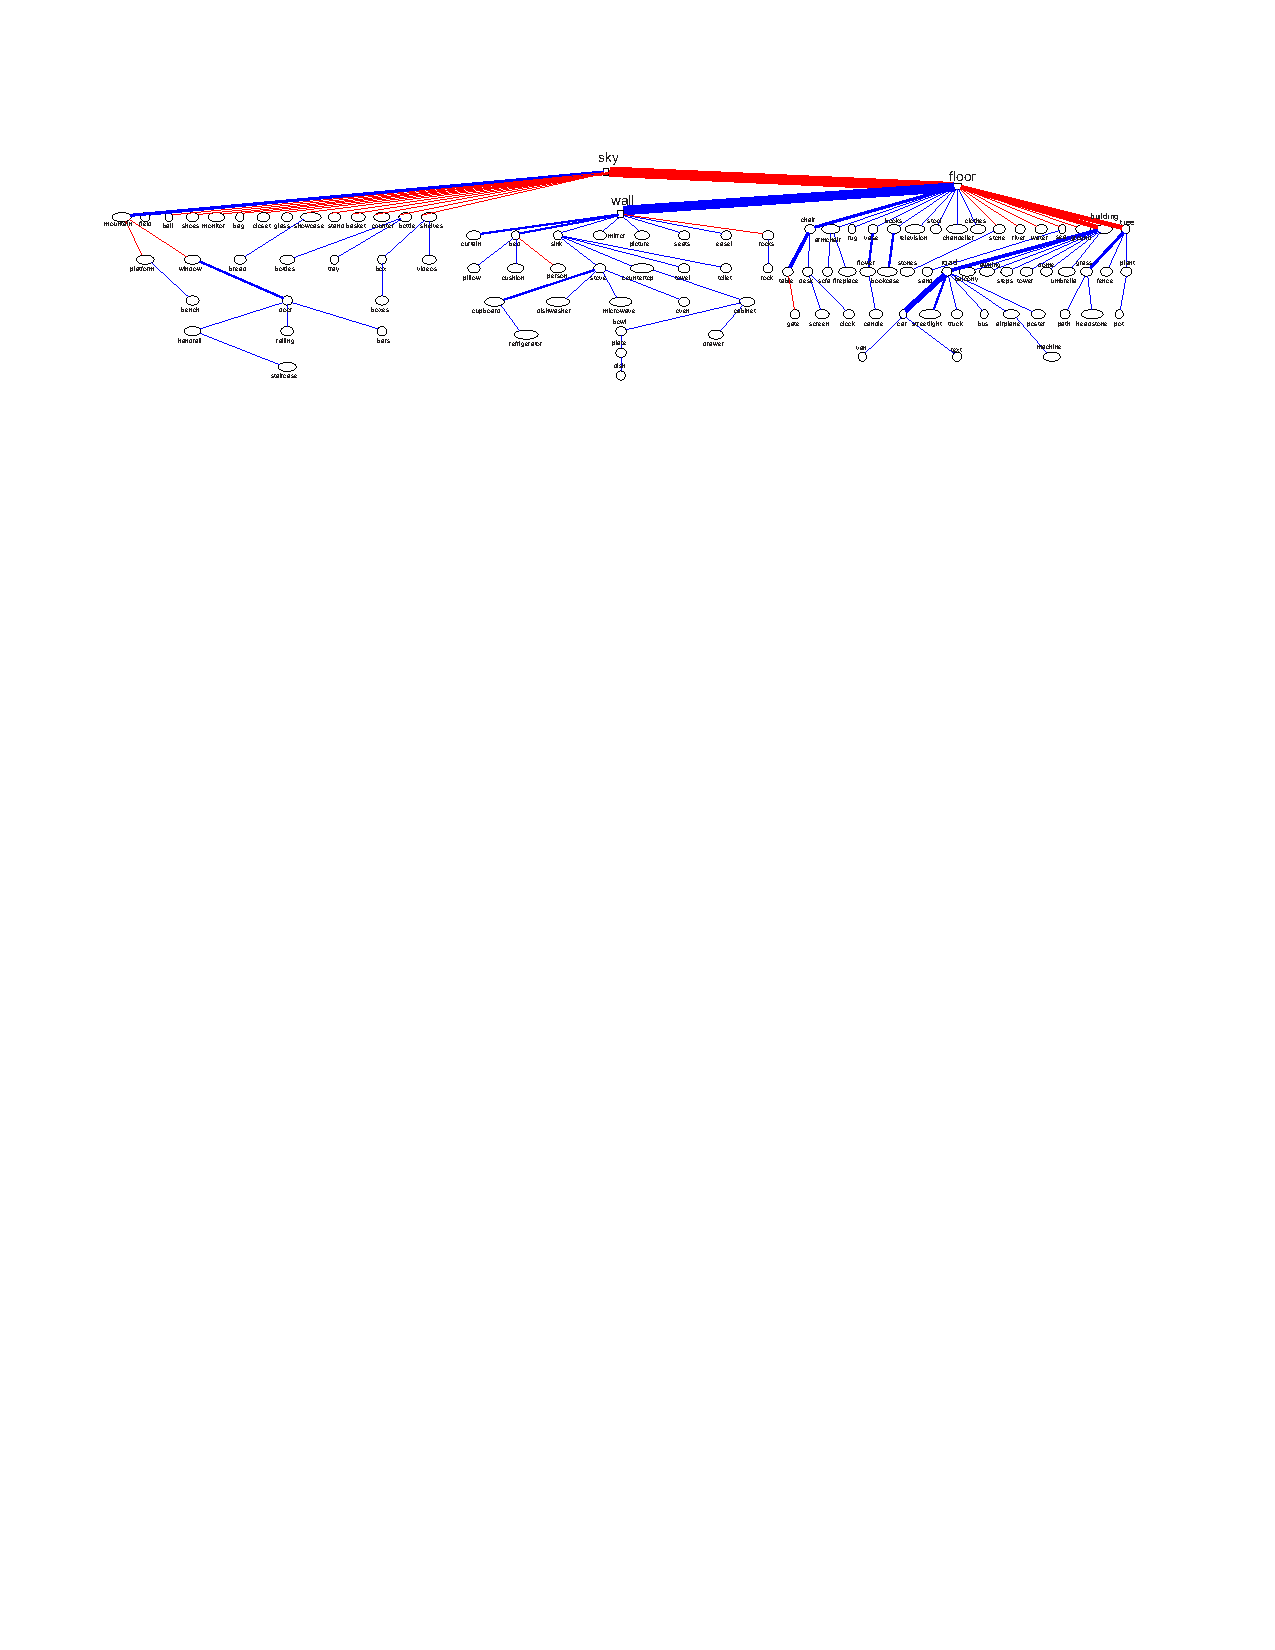
\includegraphics[width=5.8in]{object_recognition_in_context2}
\vspace{-8mm}
\caption{Pairwise MRF of object class presences in images \cite{choi_cvpr10}. Red edges denote negative correlations between classes. The thickness of each edge represents the strength of the link. You will be learning this MRF in question 3.\label{fig:object_rec2}}
\end{figure}
We can simplify the quantity being maximized over $T$ as follows (let $N=|\mathcal{D}|$):
\begin{eqnarray*}
&=&\sum_{{\bf x}\in \mathcal{D}} \Big(
\sum_{(i,j)\in T}\log\left[\frac{\hat{p}(x_i,x_j)}{\hat{p}(x_i)\hat{p}(x_j)}\right] + \sum_{j\in V}\log\left[ \hat{p}(x_j)\right]\Big)  \\
&=&\sum_{(i,j)\in T}\sum_{{\bf x}\in \mathcal{D}} \log\left[\frac{\hat{p}(x_i,x_j)}{\hat{p}(x_i)\hat{p}(x_j)}\right] + \sum_{j\in V}\sum_{{\bf x}\in \mathcal{D}}\log\left[ \hat{p}(x_j)\right]  \\
&=&\sum_{(i,j)\in T}\sum_{x_i, x_j}N\hat{p}(x_i, x_j) \log\left[\frac{\hat{p}(x_i,x_j)}{\hat{p}(x_i)\hat{p}(x_j)}\right] + \sum_{j\in V} \sum_{x_i}N\hat{p}(x_i) \log\left[ \hat{p}(x_j)\right]  \\
&=& N\Big(\sum_{(i,j)\in T} I_{\hat{p}}(X_i, X_j) - \sum_{j\in V} H_{\hat{p}}(X_j)\Big),
\end{eqnarray*}
where $I_{\hat{p}}(X_i,X_j)=\sum_{x_i,x_j} \hat{p}(x_i,x_j)\log\frac{\hat{p}(x_i,x_j)}{\hat{p}(x_i)\hat{p}(x_j)}$ is the empirical {\em mutual information} of variables $X_i$ and $X_j$, and $H_{\hat{p}}(X_i)$ is the empirical {\em entropy} of variable $X_i$. Since the entropy terms are not a function of $T$, these can be ignored for the purpose of finding the maximum likelihood tree structure. {\bf We conclude that the maximum likelihood tree can be obtained by finding the maximum-weight spanning tree in a complete graph with edge weights $I_{\hat{p}}(X_i,X_j)$ for each edge $(i,j)$}.

%Chow and Liu show that this expression is maximized by matching the sufficient statistics of $T$ with true distribution $P$
%(from data) given tree structure.
%This leads to $T(x_i,x_j)=\hat{P}(x_i,x_j)$ and $T(x_j)=\hat{P}(x_j)$. Binary term in potential function $\phi(x_i,x_j)$
%and unary term in potential function function $\phi(x_j)$ could be get from above formula directly.

%how to optimally second-order terms of the product approximation($T$) so that 
%minimize Kullback-Leibler distance ($D_{KL}(P\|T)$)
%on the actual distribution($P$), thus it is the {\it closest} approximation in information-theoretic sense. 
%The optimal dependence tree(Chow-Liu tree) that best approximates $P(x)$ is determined by $T^*=\arg\min_T D_{KL}(P\|T)$
%which is equivalent with $T^*=\arg\max_T\sum_x P(x)\log T(x)$:

The Chow-Liu algorithm then consists of the following two steps:
\begin{enumerate}
    \item Compute each edge weight based on the empirical mutual information.
    \item Find a maximum spanning tree (MST) via Kruskal or Prim's Algorithm.
    \item Output a pairwise MRF with edge potentials $\phi_{ij}(x_i,x_j) = \frac{\hat{p}(x_i,x_j)}{\hat{p}(x_i)\hat{p}(x_j)}$ for each $(i,j)\in T$ and node potentials $\phi_i(x_i) = \hat{p}(x_i)$.
\end{enumerate}
%Edge weight of edge $E(x_i,x_j)$ is defined based on mutual information $I(x_i,x_j)$:
%$$
%I(x_i,x_j)=\sum_{x_i,x_j} \hat{P}(x_i,x_j)\log\frac{\hat{P}(x_i,x_j)}{\hat{P}(x_i)\hat{P}(x_j)}
%$$
%where $\hat{P}(x_i,x_j)$ is empirical distribution of $x_i$ and $x_j$ in our data set, i.e. $\hat{P}(x_i,x_j)=count(x_i,x_j)/m$.
%$count(x_i,x_j)$ is the number of appearance of $x_i$ and $x_j$ in data set and $m$ is number of examples in total.
%For example, you want to compute $I(x_i,x_j)$:
%$$
%I(x_i,x_j)=\sum_{v_i=0}^1\sum_{v_j=0}^1 \hat{P}(x_i=v_i,x_j=v_j)\log\frac{\hat{P}(x_i=v_i,x_j=v_j)}{\hat{P}(x_i=v_i)\hat{P}(x_j=v_j)}
%$$

We have one random variable $X_i\in \{0,1\}$ for each object type (e.g., ``car'' or ``road'') specifying whether this object is present in a given image. For this problem, you are provided with a matrix of dimension $N \times M$ where $N=4367$ is the number of images in the training set and $M=111$ is the number of object types. This data is in the file ``chowliu-input.txt'', and the file ``names.txt'' specifies the object names corresponding to each column.

%If image $j$ contains object $i$, then entry $(i,j$) will be $1$, otherwise $0$. Based on such on/off matrix representation, you are going to 

Implement the Chow-Liu algorithm described above to learn the maximum
likelihood tree-structured MRF from the data provided. Your code should output the MRF in the standard UAI format described here:
\begin{center}
\url{http://www.hlt.utdallas.edu/~vgogate/uai14-competition/modelformat.html}
\end{center}


\comment
{\item Consider the Bayesian network shown below, and answer the
  following questions. You may assume that the random variables are
  binary-valued, i.e. take states in $\{0,1\}$.
\vspace{-2mm}
\begin{figure}[h]
\centering 
%\caption{}
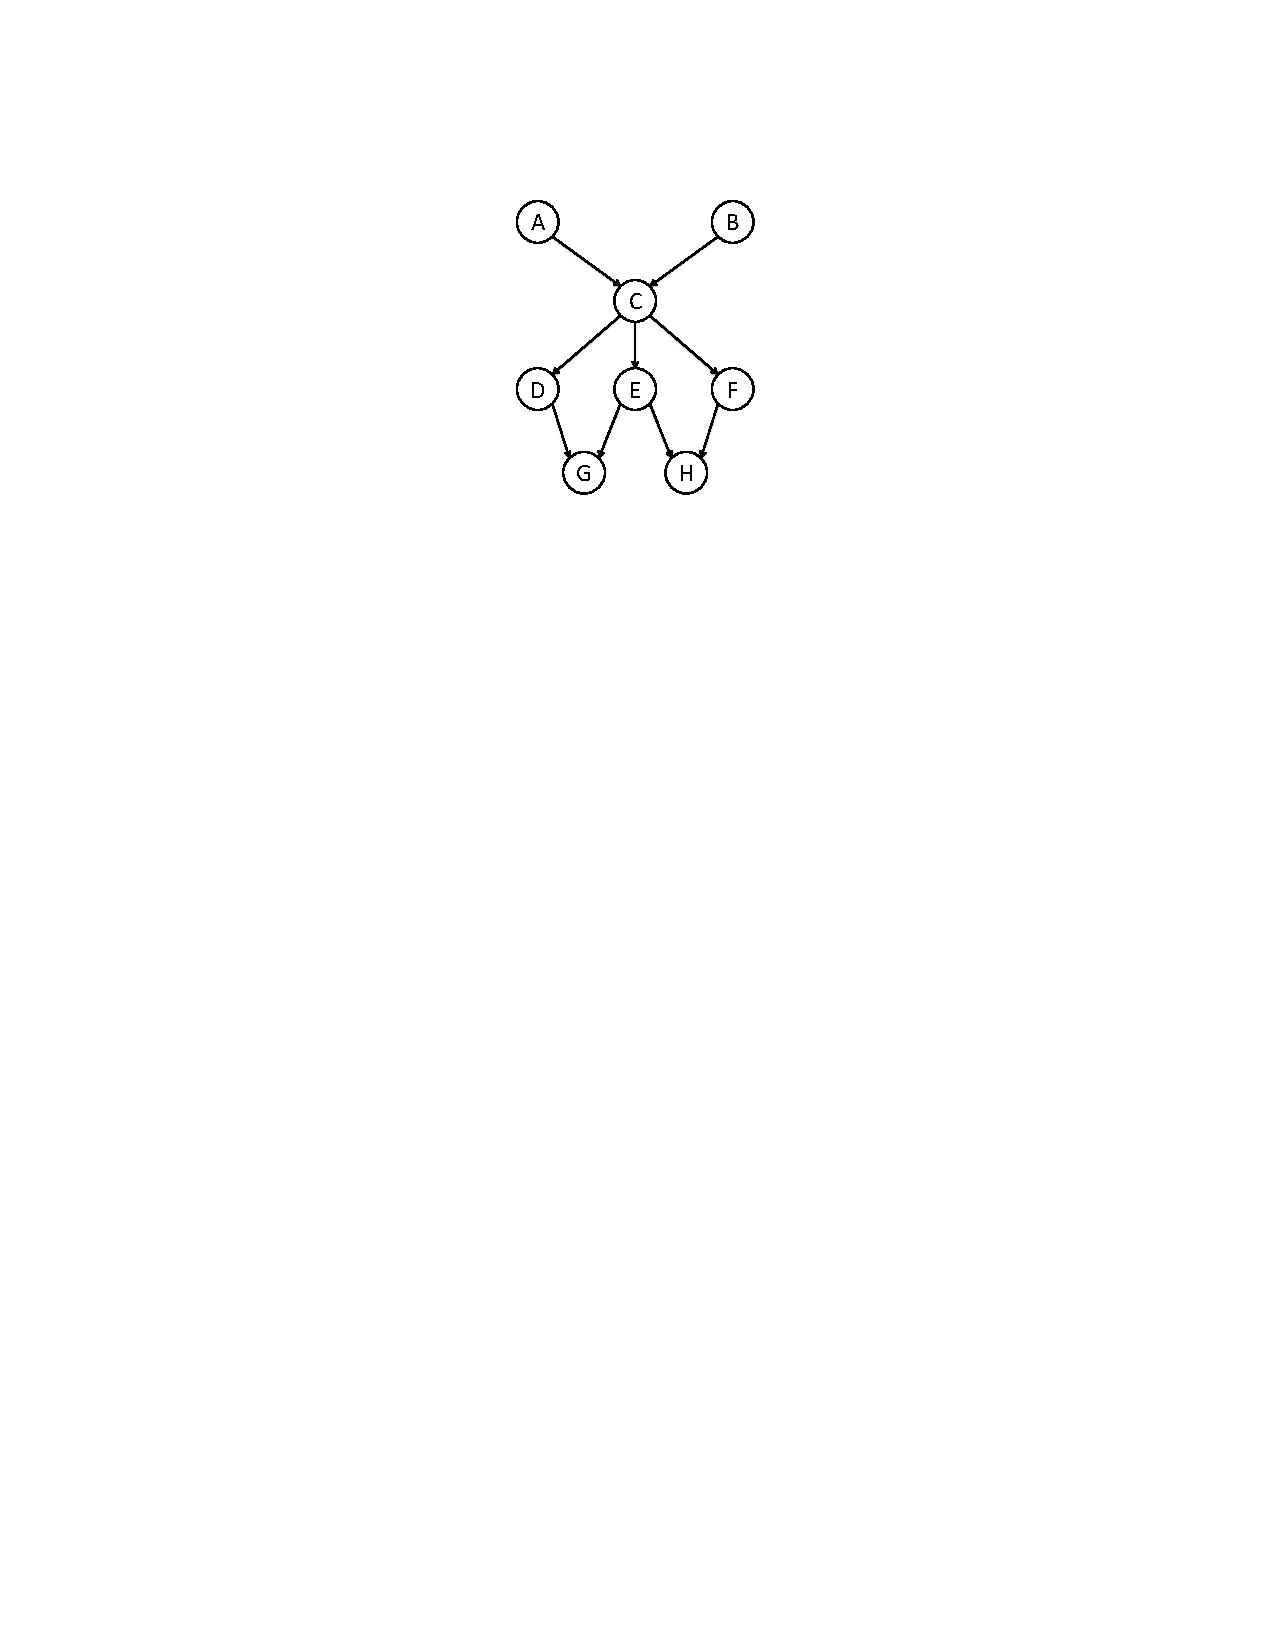
\includegraphics[width=1.5in]{eric_bn}\label{fig:eric_bn}
\end{figure}
\vspace{-6mm}
\begin{enumerate}
\item Moralize the Bayesian network (submit a drawing of the new graph). What edges are added?

{\color{blue} {\bf Answer: }
The moralized Bayes net has the following additional edges: A-B, D-E, E-F. 
}

\item Give a perfect elimination ordering, i.e. one that yields no fill edges. 

{\color{blue} {\bf Answer: }
One perfect ordering is A,B,G,H,D,F,E,C.
}

\item Give an elimination ordering that results in the induced graph
  having $\geq 5$ nodes in one (or more) cliques.

{\color{blue} {\bf Answer: }
One such ordering is E,D,G,H,F,C,A,B.
}

%\item What is the treewidth (minimal induced width) of the graph, after moralizing?
% largest clique 3, treewidth 2.

% Suppose we also had the edge $A\rightarrow G$.

%For the rest of the question, consider the original Bayesian network shown in Figure \ref{fig:eric_bn}.
\item Suppose we want to compute the query $\Pr(B=0 \mid G=1)$. 
 Prove that H and F are irrelevant variables with respect to this query. That is, show that it is possible to prune the Bayesian network, removing H and F, while not changing the value of $\Pr(B=0 \mid G=1)$.

{\color{blue} {\bf Answer: }
For a complete treatment of pruning in Bayesian networks, see this
paper:

Pruning Bayesian Networks for Efficient Computation\\
Michelle Baker, Terrance E. Boult\\
Proceedings of the Sixth Conference on Uncertainty in Artificial
Intelligence (UAI), 1990\\
\url{https://arxiv.org/abs/1304.1112}
}

%\item Is it possible to prune the Bayesian network to remove any irrelevant variables with respect to this query? Explain your answer in 1--3 sentences.

\item Walk through the execution of the variable elimination algorithm to compute $\Pr(B=0 \mid G=1)$, using as few computations as necessary (i.e., using the elimination ordering given in (b), and using the simplication given by your answer to (d)).
\end{enumerate}


\item {\bf Hidden Markov models}.
Harry lives a simple life. Some days he is Angry and some days he is
Happy. But he hides his emotional state, and so all we can observe is whether he smiles, frowns, laughs, or yells. Harry's best friend is utterly confused about whether Harry is actually happy or angry and decides to model his emotional state using a hidden Markov model.

Let $X_d\in \{$Happy, Angry$\}$ denote Harry's emotional state on day $d$, and let $Y_d \in \{$smile, frown, laugh, yell$\}$ denote the observation made about Harry on day $d$. {\bf Assume that on day 1 Harry is in the Happy state}, i.e. $X_1 = $ Happy. Furthermore, assume that Harry transitions between states exactly once per day (staying in the same state is an option) according to the following distribution: $p(X_{d+1} = $ Happy $ \mid X_d = $ Angry$) = 0.1$, $p(X_{d+1} = $ Angry $ \mid X_d = $ Happy$) = 0.1$, $p(X_{d+1} = $ Angry $ \mid X_d = $ Angry$) = 0.9$, and $p(X_{d+1} = $ Happy $ \mid X_d = $ Happy$) = 0.9$.

The observation distribution for Harry's Happy state is given by $p(Y_d
= \textrm{smile} \mid X_d = \textrm{Happy}) = 0.6, p(Y_d =
\textrm{frown} \mid X_d = \textrm{Happy}) = 0.1, p(Y_d =
\textrm{laugh} \mid X_d = \textrm{Happy}) = 0.2$, and $p(Y_d =
\textrm{yell} \mid X_d = \textrm{Happy}) = 0.1$. The observation
distribution for Harry's Angry state is  $p(Y_d = \textrm{smile} \mid
X_d = \textrm{Angry}) = 0.1, p(Y_d = \textrm{frown} \mid X_d =
\textrm{Angry}) = 0.6, p(Y_d = \textrm{laugh} \mid X_d =
\textrm{Angry}) = 0.1$, and $p(Y_d = \textrm{yell} \mid X_d =
\textrm{Angry}) = 0.2$.

\vspace{2mm}
{\bf All of this is summarized in the following figure}:
\vspace{-1mm}
\begin{center}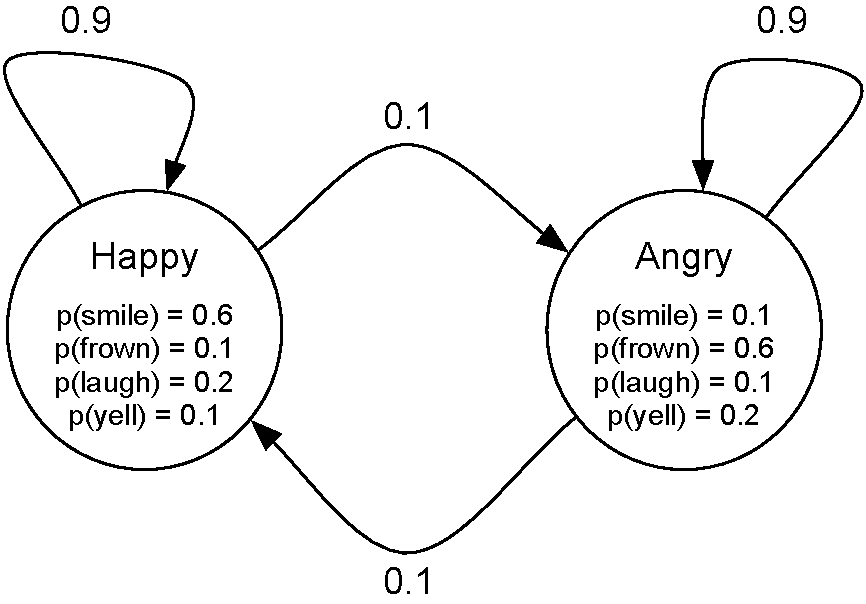
\includegraphics[width=235pt]{../ps1/hmm_fig}\end{center}
\vspace{-2mm}
{\bf Be sure to show all of your work for the below questions.} Note,
the goal of this question is to get you to start thinking deeply about
probabilistic inference. Thus, although you could look at Chapter 17
for an overview of HMMs, try to solve this question based on first
principles (also: no programming needed!).
\begin{enumerate}

\item What is $p(X_2 = \textrm{Happy})$?
\item What is $p(Y_2 = \textrm{frown})$?
\item What is $p(X_2 = \textrm{Happy} \mid Y_2 = \textrm{frown})$?
\item What is $p(Y_{80} = \textrm{yell})$?
\item Assume that $Y_1 = Y_2 = Y_3 = Y_4 = Y_5 = \textrm{frown}$. What is the most likely sequence of the states? That is, compute the MAP assignment $\arg\max_{x_1, \ldots, x_5} p(X_1=x_1, \ldots, X_5=x_5 \mid Y_1 = Y_2 = Y_3 = Y_4 = Y_5 = \textrm{frown})$.

\end{enumerate}
}


\comment{
\item 
% From Berkeley, A_hw5_Fa11.tex
%\begin{center}{\bf \large  HMM with mixture model emissions}\end{center}

A common modification of the hidden Markov model involves using mixture models for the
emission probabilities $p(\yy_t | q_t)$, where $q_t$ refers to the state for time $t$ and $\yy_t$ to the observation for time $t$.

Suppose that ${\bf y}_t \in \real^n$ and that the emission distribution is given by a mixture of Gaussians for each value of the state. To be concrete, suppose that the $q_t$ can take $K$ discrete states and each mixture has $M$ components. Then,
\[
p({\bf y}_t \mid q_t) = \sum_{j=1}^M b_{q_t j}
\left(\frac{1}{(2\pi)^{\frac{n}{2}}|\Sigma_{q_t j}|^{\frac{1}{2}}}
\exp\left\{-\frac{1}{2}({\bf y}_t-\mu_{q_t j})^T\Sigma_{q_t j}^{-1}({\bf y}_t-\mu_{q_t j})
\right\}\right)
\]
where ${\bf b}_i \in [0,1]^M$ denotes the mixing weights for state $i$ ($\sum_{j=1}^M b_{ij} = 1$ for $i=1,\ldots K$), $\mu_{ij} \in  \real^n$ and $\Sigma_{ij} \in  \real^{n\times n}$.

Let $\pi \in \real^K$ be the probability distribution for the initial state $q_0$,
and $A \in \real^{K \times K}$ be the transition matrix of the $q_t$'s.
In this problem you will derive an EM algorithm for learning the parameters $\{ b_{ij}, \mu_{ij}, \Sigma_{ij} \}$ and $A, \pi$.

\begin{enumerate}
\item The EM algorithm is substantially simpler if you introduce auxiliary variables $z_t\in \{1, \ldots, M\}$ denoting which mixture component the $t$'th observation is drawn from.

Draw the graphical model for this modified HMM, identifying
  clearly the additional latent variables that are needed.
\item Write the expected complete log likelihood for the model
  and identify the expectations that you need to compute in the E
  step. {\em Show all steps of your derivation.}

\item Give an algorithm for computing the E step.

{\em Hint: Reduce the inference problem to something you know how to do, such as sum-product belief propagation in tree-structured pairwise MRFs.}

\item Write down the equations that implement the M step.
\end{enumerate}
}



\end{enumerate}


\bibliographystyle{plain}
\bibliography{../../defs}


\end{document}
